\documentclass{article}

\usepackage[ngerman]{babel}
\usepackage[utf8]{inputenc}
\usepackage[T1]{fontenc}
\usepackage{hyperref}
\usepackage{csquotes}
\usepackage{graphicx}
\usepackage{float}
\usepackage{caption}

\usepackage[
    backend=biber,
    style=apa,
    sortlocale=de_DE,
    natbib=true,
    url=false,
    doi=false,
    sortcites=true,
    sorting=nyt,
    isbn=false,
    hyperref=true,
    backref=false,
    giveninits=false,
    eprint=false]{biblatex}
\addbibresource{../references/bibliography.bib}

\title{Notizen zum Projekt Data Ethics}
\author{Noah Cooper}
\date{\today}

\begin{document}
\maketitle

\abstract{
    Dieses Dokument ist eine Sammlung von Notizen zu dem Projekt. Die Struktur innerhalb des
    Projektes ist gleich ausgelegt wie in der Hauptarbeit, somit kann hier einfach geschrieben
    werden, und die Teile die man verwenden möchte, kann man direkt in die Hauptdatei ziehen.
}

\tableofcontents

\newpage

\section{Leitfrage}
    Ist es ethisch vertretbar, KI für die Erstellung von Kunst zu verwenden?

\section{Einführung}
    Künstliche Intelligenz hat die Welt im Sturm erobert. Völlig logisch, denn sie arbeitet noch 
    personalisierter und effizienter als eine einfache Suchmaschine, was in unserer heutigen Gesellschaft 
    sehr gefragt ist. Auch im Bereich der Kunst sieht es nicht anders aus. Aber wem gehören die Urheberechte, wenn hinter einer Kreation gar kein Mensch steckt? Und welche Auswirkungen kann das auf unser aktuelles Verständnis der Kunst haben?


\section{Wie wird KI trainiert?}
    Laut yukosai.com kann das Training einer KI in mehrere Schritte unterteilt werden:
    \begin{enumerate}
        \item Vorbereitung der Trainingsdaten: Auswahl einer großen Anzahl von Bildern als Basis für das Training.
        \item Labeling der Daten: Jedes Bild wird mit entsprechenden Labels versehen, um dem Modell mitzuteilen, welcher Stil oder welches Genre repräsentiert wird.
        \item Aufbau des neuronalen Netzwerks: Das Modell wird so konfiguriert, dass es die gewünschten künstlerischen Merkmale erlernen kann.
        \item Training des Modells: Durch mehrere Iterationen werden die Gewichte im Netzwerk angepasst, um die Genauigkeit und Qualität der generierten Kunstwerke zu verbessern.
        \item Auswertung und Anpassung: Nach dem Training wird das Modell auf seine Leistung überprüft und gegebenenfalls weiter optimiert.
    \end{enumerate}
    (hier noch mehr schreiben zu kein kreatives Denken, pattern recognition)
    

    \subsection{Wie gut ist die KI-Kunst?}
        Mit einem AI Image Generator lässt sich jedes Bild erstellen, dass man sich nur wünschen könnte. 
        An Qualität lassen sie aber oft zu wünschen übrig. 
        KI Kunst kann sehr verstörend sein, was das Beispielbild weiter unten zeigt: Auf den ersten Blick sieht es aus wie ein mystisches oder märchenhaftes Bild von einer Elfe, die von merkwürdigen Gestalten verfolgt wird. Diese Idee wird einem auch sehr gut vom Bild vermittelt. Sobald man aber genauer hinsieht, merkt man, dass die Proportionen überhaupt nicht passen: Des Mädchens Finger wachsen an komischen Stellen aus ihren Händen; ihre Ohren sehen total komisch aus und ihr Hals ist eigentlich gar nicht vorhanden. Die Gestalten hinter ihr haben zum Beispiel drei Augen oder man erkennt gar nicht, wo ihre Nase ist. Dieses Beispiel zeigt, dass die heutige KI eindeutig nicht dazu in der Lage ist, realistische Kunst zu erstellen.
        \begin{figure}[ht]
        \centering
        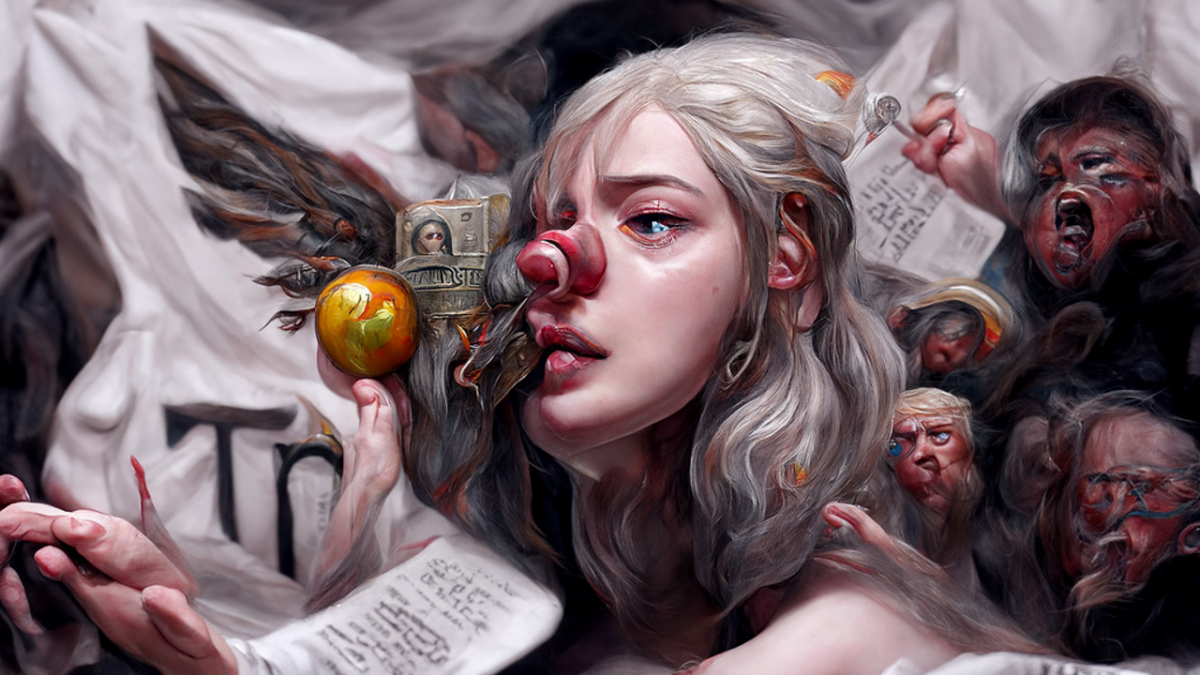
\includegraphics[width=0.8\textwidth]{ki-bild.png} 
        \caption{A detailed painting of an allegory of truth and lies - Disco Diffusion (Versuch 55)}
        \label{fig:ki-bild}
        \end{figure}
    
        Die KI ist ausserdem gar nicht so lernfähig, wie man vielleicht denken würde. Laut golem.de befindet sie sich ungefähr auf diesem Stand: "Während ein Kind nach dem Ansehen und Lernen des Inhaltes Katze sehr schnell jede Katze in jeder möglichen Position – zum Beispiel mit gedrehtem Kopf – identifizieren kann, würde das Netzwerk gnadenlos scheitern, wenn die Trainingsdaten keine Bilder von Katzen in Profilansicht enthielten." \Citep{ki-krempelt-die-kunst-um}

\section{Was sagen Befürworter*innen der KI-Kunst?}
    Die künstliche Intelligenz kann helfen, Kunst und Kultur zugänglicher zu machen und die kreativen 
    Prozesse von Kunstschaffenden zu unterstützen und zu beschleunigen. \Citep{unesco} Sie passt sich auch komplett an die Bedarfe und Wünsche ihrer Nutzer*innen an: KI kann jeden Auftrag entgegennehmen und bearbeiten. Dadurch sind viele Leute der Meinung, die KI erleichtere ihren Alltag und helfe ihnen, schnell zu Antworten zu kommen.

\section{Risiken und Fragen über Urheberechte}
    Da die KI nicht selber denken, sondern nur mit bereits prozessierten Daten arbeiten kann, verwendet sie viele urheberechtlich geschützte Dokumente. Auf Social Media gibt es hunderte von Accounts, die KI-generierte Bilder posten und dafür viel Aufmerksamkeit und Bewunderung bekommen (z.B. @troplanduniverse). Das lässt bei Einigen aber einen bitteren Nachgeschmack, weil sie finden, dass es so viele Künstler*innen gibt, die viel Energie, Geld, Zeit und Leidenschaft in ihre Kunst stecken, nur um dann in der Masse unterzugehen. Und weil die KI keine Quellen angibt, ist es schwierig nachzuweisen, wenn und ob sie ein Bild einer anderen Person geklaut hat. 
    (Ki-Kunst ist nicht sehr wertvoll, weil sie unlimitiert sind)

\section{Meine eigene Meinung vor der Recherche}
    Mit der KI lassen sich viele interessante Kunstwerke erstellen, wie man anhand von Ai Image 
    Generators erkennen kann. Ich kann mir aber vorstellen, dass viele Künstler*innen eine Gefahr 
    darin sehen, dass ihre Arbeitsplätze und ihre Einnahmequelle verschwinden könnten. Die Kunst der KI 
    hat in meinen Augen ohne den Aspekt der menschlichen Überlegungen nicht so viel Wert. Die KI denkt 
    sich nicht aus, welche Nachricht sie mit ihrer Kunst teilen will, weshalb man sie auch nicht 
    interpretieren und darüber diskutieren kann.

\section{Fazit}
    Die Verwendung von KI hat in jedem Bereich positive und negative Aspekte. In der Kunst ist sie jedoch 
    besonders kontrovers, weil für viele Leute der menschliche Aspekt eine grosse Rolle spielt.
    (Auf Fragen aus der Einleitung und Leitfrage antworten)

\input{section_ai.tex}

\printbibliography

\end{document}
